\chapter{Demolevel}
Zu Anfang des Projekts war die Gestaltung und der Aufbau des Levels durch Sprites gedacht, die den Hintergrund darstellen sollten. Durch Probleme mit Skalierungen und wiederholenden Hintergr"unden waren wir gezwungen das Level unlogisch aufzubauen. So mussten wir zum Beispiel viele Kisten stapeln um eine weitere Ebene zu erreichen, was nicht in die Szene gepasst h"atte. Deshalb haben wir uns entschieden das Level durch Tiles zu gestalten. Zu Erstellung nutzten wir das Programm "Tiled" sowie "Tiled2Unity" zum importieren in Unity. Dabei wurden freie Tilesets genutzt.

\begin{figure}
	\centering
	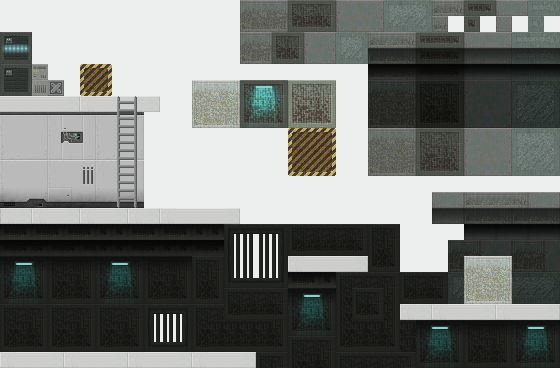
\includegraphics[height=5cm]{images/tileset.jpg}
	\caption{F"ur das Level genutztes Tileset}
	\label{fig:screen_pre}
\end{figure}


Das Level sollte zu Beginn schon einem Turm "ahneln, um an der Spitze den Kampf gegen den Endgegner einzuf"ugen. Ziel beim bauen des Levels war es den Spieler dazu zu bringen alle seine F"ahigkeiten zu nutzen um, m"oglichst unbeschadet, ans Ende des Levels zu kommen und den Endgegner zu besiegen.
Um den Spieler an die Steuerung zu gew"ohnen wird er schon fr"uh mehrere Spr"unge vollf"uhren m"ussen um in den n"achsten Abschnitt zu gelangen. Damit der Spieler nicht st"andig von einer Einer ebene zur n"achsten Springen muss wurden die "Luftstr"ome" eingef"uhrt, die ihn automatisch nach Oben tragen. Um diese darzustellen wurde ein Partikeleffekt genutzt.


\begin{lstlisting}[breaklines=true]
	[...]
	//befindet sich der Spieler innerhalb des Colliders des Luftstrom, so wird ihm in Richtung der
	// y-Achse geschwindigkeit hinzgefuegt
	void OnTriggerStay2D(Collider2D other)
	{
		if(other.tag == "Player")
			other.attachedRigidbody.velocity = new Vector2 (other.attachedRigidbody.velocity.x, other.attachedRigidbody.velocity.y+0.3f);
	}
\end{lstlisting}

Weiterhin wurden T"uren und Aufz"uge genutzt um den Spieler gro"se Abschnitte weiter nach oben Steigen oder ihn ins innere des Turms wechseln zu lassen. Daf"ur wurde ein Script genutzt das aktiviert wird sobald der Spieler innerhalb des Colliders "e" dr"uckt. Dadurch f"arbt sich der Bildschirm schwarz und der Spieler sowie die Kamera wird zur Ausgangst"ur bewegt. Danach klart der Bildschirm wieder auf.

\begin{lstlisting}[breaklines = true]
	[...]
	void OnTriggerStay2D(Collider2D other)
	{
		if (other.tag == "Player" && Input.GetKeyDown ("e") && !isFading) {
			isFading = true;
			fadeToBlack = true;
		}
	}
	
	//Zum aufklaren des Bildschirms
	//Lerpt zwischen der momentanen Farbe der Textur und "Klar" bis der Alphawert der Textur kleiner als 0.1 ist.
	//Danach wird die Farbe auf "Klar" gesetzt.
	void FadeToClear()
	{ 
		fadeTexture.color = Color.Lerp (fadeTexture.color, Color.clear, 1.5f * Time.deltaTime);
		if(fadeTexture.color.a <= 0.1f)
		{
			fadeTexture.color = Color.clear;
			fadeTexture.enabled = false;
			isFading = false;
		}
	}
	
	//Um den Bildschirm schwarz zu faerben
	//Lerpt zwischen der momentanen Farbe der Textur und "Schwarz" bis der Alphawert der Textur groesser als 0.8 ist.
	//Danach wird die Farbe auf "Schwarz" gesetzt.
	void FadeToBlack()
	{
		fadeTexture.enabled = true;
		fadeTexture.color = Color.Lerp (fadeTexture.color, Color.black, 1.5f * Time.deltaTime);
		if (fadeTexture.color.a >= 0.8f) {
			fadeTexture.color = Color.black;
			fadeToBlack = false;
			playerTransform.position = target.position;
			cam.position = new Vector3 (target.position.x, target.position.y, cam.position.z);
		}
	}